\documentclass[12pt,]{article}
\usepackage{lmodern}
\usepackage{amssymb,amsmath}
\usepackage{ifxetex,ifluatex}
\usepackage{fixltx2e} % provides \textsubscript
\ifnum 0\ifxetex 1\fi\ifluatex 1\fi=0 % if pdftex
  \usepackage[T1]{fontenc}
  \usepackage[utf8]{inputenc}
\else % if luatex or xelatex
  \ifxetex
    \usepackage{mathspec}
  \else
    \usepackage{fontspec}
  \fi
  \defaultfontfeatures{Ligatures=TeX,Scale=MatchLowercase}
\fi
% use upquote if available, for straight quotes in verbatim environments
\IfFileExists{upquote.sty}{\usepackage{upquote}}{}
% use microtype if available
\IfFileExists{microtype.sty}{%
\usepackage{microtype}
\UseMicrotypeSet[protrusion]{basicmath} % disable protrusion for tt fonts
}{}
\usepackage[margin=1in]{geometry}
\usepackage{hyperref}
\hypersetup{unicode=true,
            pdftitle={Death Rate Data Investigation},
            pdfauthor={Pieter Janse van Rensburg},
            pdfborder={0 0 0},
            breaklinks=true}
\urlstyle{same}  % don't use monospace font for urls
\usepackage{color}
\usepackage{fancyvrb}
\newcommand{\VerbBar}{|}
\newcommand{\VERB}{\Verb[commandchars=\\\{\}]}
\DefineVerbatimEnvironment{Highlighting}{Verbatim}{commandchars=\\\{\}}
% Add ',fontsize=\small' for more characters per line
\usepackage{framed}
\definecolor{shadecolor}{RGB}{248,248,248}
\newenvironment{Shaded}{\begin{snugshade}}{\end{snugshade}}
\newcommand{\KeywordTok}[1]{\textcolor[rgb]{0.13,0.29,0.53}{\textbf{#1}}}
\newcommand{\DataTypeTok}[1]{\textcolor[rgb]{0.13,0.29,0.53}{#1}}
\newcommand{\DecValTok}[1]{\textcolor[rgb]{0.00,0.00,0.81}{#1}}
\newcommand{\BaseNTok}[1]{\textcolor[rgb]{0.00,0.00,0.81}{#1}}
\newcommand{\FloatTok}[1]{\textcolor[rgb]{0.00,0.00,0.81}{#1}}
\newcommand{\ConstantTok}[1]{\textcolor[rgb]{0.00,0.00,0.00}{#1}}
\newcommand{\CharTok}[1]{\textcolor[rgb]{0.31,0.60,0.02}{#1}}
\newcommand{\SpecialCharTok}[1]{\textcolor[rgb]{0.00,0.00,0.00}{#1}}
\newcommand{\StringTok}[1]{\textcolor[rgb]{0.31,0.60,0.02}{#1}}
\newcommand{\VerbatimStringTok}[1]{\textcolor[rgb]{0.31,0.60,0.02}{#1}}
\newcommand{\SpecialStringTok}[1]{\textcolor[rgb]{0.31,0.60,0.02}{#1}}
\newcommand{\ImportTok}[1]{#1}
\newcommand{\CommentTok}[1]{\textcolor[rgb]{0.56,0.35,0.01}{\textit{#1}}}
\newcommand{\DocumentationTok}[1]{\textcolor[rgb]{0.56,0.35,0.01}{\textbf{\textit{#1}}}}
\newcommand{\AnnotationTok}[1]{\textcolor[rgb]{0.56,0.35,0.01}{\textbf{\textit{#1}}}}
\newcommand{\CommentVarTok}[1]{\textcolor[rgb]{0.56,0.35,0.01}{\textbf{\textit{#1}}}}
\newcommand{\OtherTok}[1]{\textcolor[rgb]{0.56,0.35,0.01}{#1}}
\newcommand{\FunctionTok}[1]{\textcolor[rgb]{0.00,0.00,0.00}{#1}}
\newcommand{\VariableTok}[1]{\textcolor[rgb]{0.00,0.00,0.00}{#1}}
\newcommand{\ControlFlowTok}[1]{\textcolor[rgb]{0.13,0.29,0.53}{\textbf{#1}}}
\newcommand{\OperatorTok}[1]{\textcolor[rgb]{0.81,0.36,0.00}{\textbf{#1}}}
\newcommand{\BuiltInTok}[1]{#1}
\newcommand{\ExtensionTok}[1]{#1}
\newcommand{\PreprocessorTok}[1]{\textcolor[rgb]{0.56,0.35,0.01}{\textit{#1}}}
\newcommand{\AttributeTok}[1]{\textcolor[rgb]{0.77,0.63,0.00}{#1}}
\newcommand{\RegionMarkerTok}[1]{#1}
\newcommand{\InformationTok}[1]{\textcolor[rgb]{0.56,0.35,0.01}{\textbf{\textit{#1}}}}
\newcommand{\WarningTok}[1]{\textcolor[rgb]{0.56,0.35,0.01}{\textbf{\textit{#1}}}}
\newcommand{\AlertTok}[1]{\textcolor[rgb]{0.94,0.16,0.16}{#1}}
\newcommand{\ErrorTok}[1]{\textcolor[rgb]{0.64,0.00,0.00}{\textbf{#1}}}
\newcommand{\NormalTok}[1]{#1}
\usepackage{longtable,booktabs}
\usepackage{graphicx,grffile}
\makeatletter
\def\maxwidth{\ifdim\Gin@nat@width>\linewidth\linewidth\else\Gin@nat@width\fi}
\def\maxheight{\ifdim\Gin@nat@height>\textheight\textheight\else\Gin@nat@height\fi}
\makeatother
% Scale images if necessary, so that they will not overflow the page
% margins by default, and it is still possible to overwrite the defaults
% using explicit options in \includegraphics[width, height, ...]{}
\setkeys{Gin}{width=\maxwidth,height=\maxheight,keepaspectratio}
\IfFileExists{parskip.sty}{%
\usepackage{parskip}
}{% else
\setlength{\parindent}{0pt}
\setlength{\parskip}{6pt plus 2pt minus 1pt}
}
\setlength{\emergencystretch}{3em}  % prevent overfull lines
\providecommand{\tightlist}{%
  \setlength{\itemsep}{0pt}\setlength{\parskip}{0pt}}
\setcounter{secnumdepth}{5}
% Redefines (sub)paragraphs to behave more like sections
\ifx\paragraph\undefined\else
\let\oldparagraph\paragraph
\renewcommand{\paragraph}[1]{\oldparagraph{#1}\mbox{}}
\fi
\ifx\subparagraph\undefined\else
\let\oldsubparagraph\subparagraph
\renewcommand{\subparagraph}[1]{\oldsubparagraph{#1}\mbox{}}
\fi

%%% Use protect on footnotes to avoid problems with footnotes in titles
\let\rmarkdownfootnote\footnote%
\def\footnote{\protect\rmarkdownfootnote}

%%% Change title format to be more compact
\usepackage{titling}

% Create subtitle command for use in maketitle
\newcommand{\subtitle}[1]{
  \posttitle{
    \begin{center}\large#1\end{center}
    }
}

\setlength{\droptitle}{-2em}
  \title{Death Rate Data Investigation}
  \pretitle{\vspace{\droptitle}\centering\huge}
  \posttitle{\par}
  \author{Pieter Janse van Rensburg}
  \preauthor{\centering\large\emph}
  \postauthor{\par}
  \predate{\centering\large\emph}
  \postdate{\par}
  \date{14 February 2018}


\begin{document}
\maketitle

{
\setcounter{tocdepth}{2}
\tableofcontents
}
\newpage

\section{Introduction}\label{introduction}

The aim of this report is to investigate various covariates believed to
affect the Death Rate (per 1000 residents) in small American Cities (see
Houghton Mifflin Harcourt, 2018). It will open with an explanatory
analysis of the data. This will be followed by the fitting of a
regression model to the data and the scrutinizing of the residuals of
the model to ensure that all theoretical assumptions have been adhered
to adequately. Lastly, the report will use Bootstrapping to explore the
distributions of the estimated coefficients of the model to analyse
their sensitivities with respect to changes in the data.

\section{Explanatory Data Analysis}\label{explanatory-data-analysis}

\begin{center}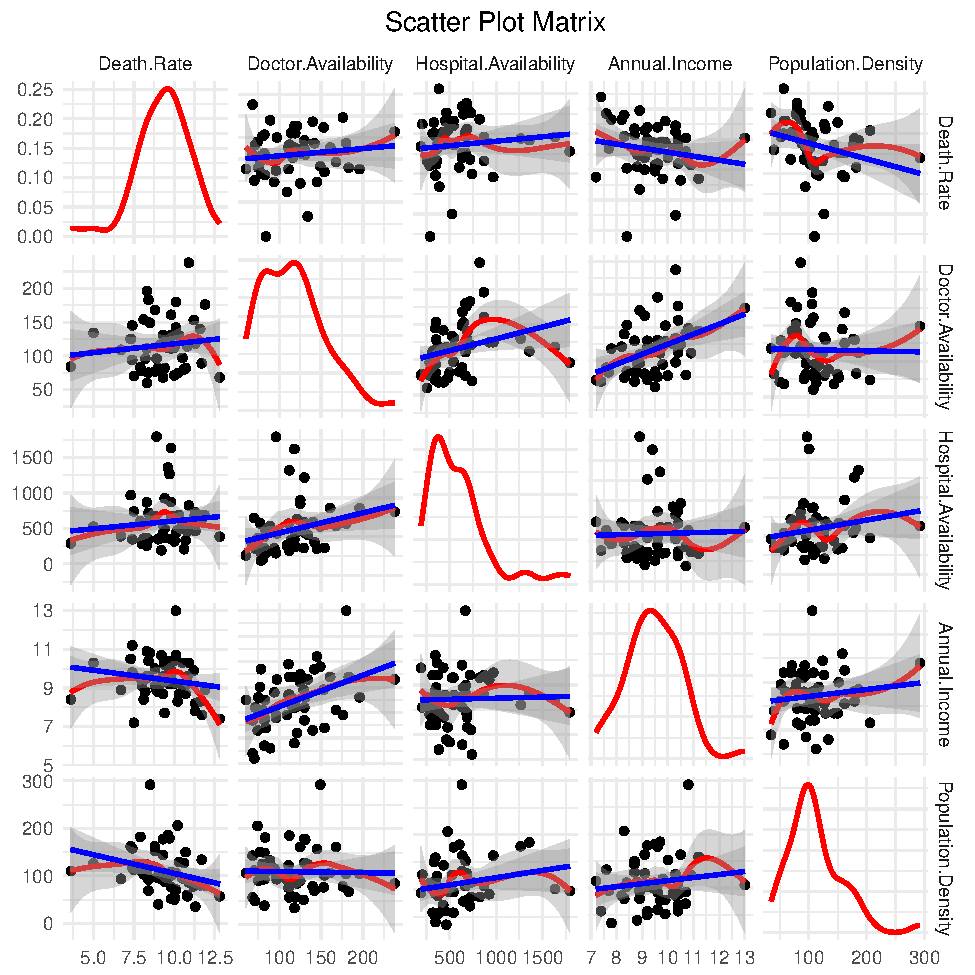
\includegraphics{report_files/figure-latex/spm_data-1} \end{center}

As can be seen by the above Scatter Plot Matrix of the data, all
covariates appear to be linearly correlated with the response variable
(\texttt{Death.Rate}). However, there also appears to be collinearities
amongst all the covariates which could lead to problems in the model
fitting procedure. Furthermore, due to linear nature of the
relationships between the response and the covariates as well as the
response's continuous scale, a linear regression model appears to be a
suitable choice to model the response variable.

\section{All Subsets Regression}\label{all-subsets-regression}

In order to select which variables should be used to model the response,
All Subsets Regression will be performed using the minimization of BIC
as the criteria of the algorithm.

\subsection{Code to Perform All Subsets
Regression}\label{code-to-perform-all-subsets-regression}

\begin{Shaded}
\begin{Highlighting}[]
\KeywordTok{library}\NormalTok{(leaps)}
\CommentTok{# Perform all subsets regression}
\NormalTok{leaps.output <-}\StringTok{ }\KeywordTok{regsubsets}\NormalTok{(Death.Rate }\OperatorTok{~}\StringTok{ }\NormalTok{Doctor.Availability }\OperatorTok{+}
\StringTok{                           }\NormalTok{Hospital.Availability }\OperatorTok{+}\StringTok{ }\NormalTok{Annual.Income }\OperatorTok{+}
\StringTok{                           }\NormalTok{Population.Density,}
                           \DataTypeTok{data =}\NormalTok{ health.dat,}
                           \DataTypeTok{nbest =} \DecValTok{1}\NormalTok{,}
                           \DataTypeTok{nvmax =} \OtherTok{NULL}\NormalTok{,}
                           \DataTypeTok{force.in =} \OtherTok{NULL}\NormalTok{,}
                           \DataTypeTok{force.out =} \OtherTok{NULL}\NormalTok{,}
                           \DataTypeTok{intercept =} \OtherTok{TRUE}\NormalTok{,}
                           \DataTypeTok{method =} \StringTok{"exhaustive"}\NormalTok{)}
\end{Highlighting}
\end{Shaded}

The above code performs All Subsets Regression to select variables for
the model using an exhaustive technique (i.e.~all possible models are
tested). The output of the algorithm is stored in the variable
\texttt{leaps.output}.

\subsection{Output of the Algorithm}\label{output-of-the-algorithm}

\begin{center}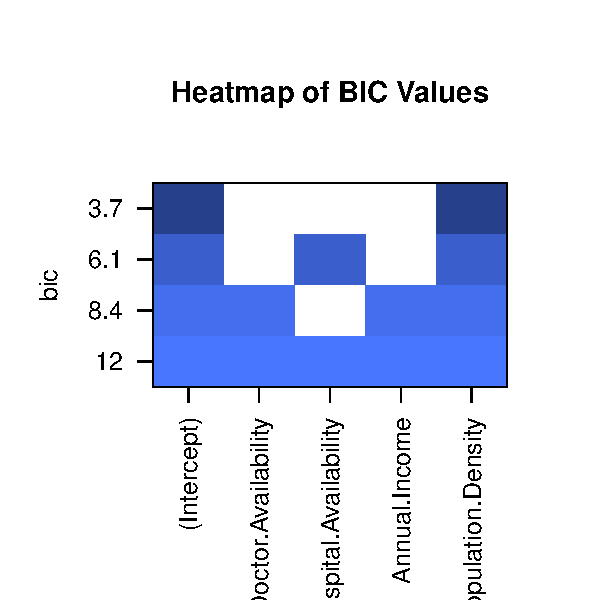
\includegraphics{report_files/figure-latex/bic_all_ss-1} \end{center}

The above heat map indicates that BIC is minimized when an intercept
term as well as the covariate \texttt{Population.Density} are used to
model the response.

\section{Fitting the Linear Model}\label{fitting-the-linear-model}

\subsection{Model Equations}\label{model-equations}

Based on the output of all subsets regression, the fitted model can be
expressed by the following equation:

\[
\begin{aligned}
 Y_{Death Rate} &=  \beta_0 + \beta_1 X_{Doctor Availability}  +  \varepsilon,\\
\text{where }  \varepsilon &\sim N(0,\ \sigma^2)
\end{aligned}
\] \newpage

\subsection{Coefficients of the fitted
model}\label{coefficients-of-the-fitted-model}

\begin{longtable}[]{@{}lrrrr@{}}
\caption{Fitted Values and their Statistics for the Fitted
Model}\tabularnewline
\toprule
& Estimate & Std. Error & t value &
Pr(\textgreater{}\textbar{}t\textbar{})\tabularnewline
\midrule
\endfirsthead
\toprule
& Estimate & Std. Error & t value &
Pr(\textgreater{}\textbar{}t\textbar{})\tabularnewline
\midrule
\endhead
(Intercept) & 10.3879974 & 0.5693501 & 18.245360 &
0.0000000\tabularnewline
Population.Density & -0.0097824 & 0.0047404 & -2.063621 &
0.0441603\tabularnewline
\bottomrule
\end{longtable}

As can be seen by the above parameter estimates, a small American city
with a population density of 0 will be expected to have \(10.38...\)
deaths per 1000 people.

Furthermore, it also appears that as the population density increases by
1 unit, the death rate can be expected to decreases by \(-0.00978...\)
per 1000 people. This is largely due to larger cities having access to
more medical services and practitioners than smaller ones (which are
usually limited to only having one clinic or practise per town).

\section{Residual Analysis}\label{residual-analysis}

\begin{center}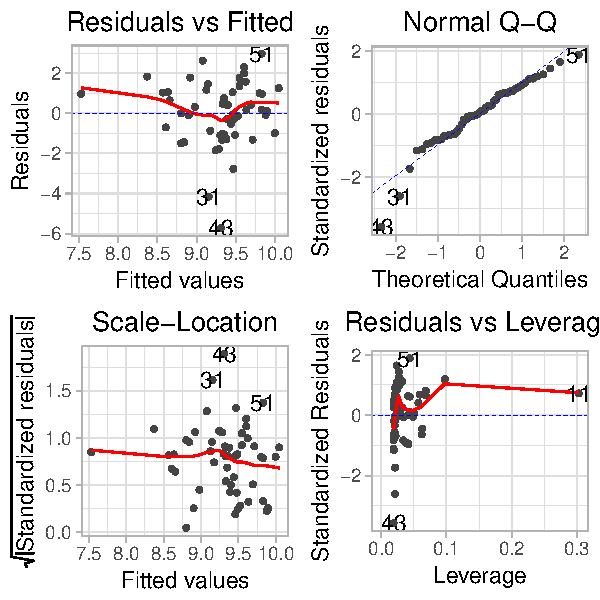
\includegraphics{report_files/figure-latex/mod_resid_analysis-1} \end{center}

As indicated by the above Residuals vs.~Fitted Plot, the assumption of 0
Residual mean appears to have been adequately met. Furthermore, the
variance of the Residuals appear to be homoskedastic once outliers
values are not considered. Additionally, the Scale-Location Plot further
emphasizes the homoskedasticity of the residuals' variance.

Based on the Normal Q-Q Plot, the assumption of Residual Normality also
appears to have been adequately met, however, there appears to be
deviations from Normality at the tails of the distribution.

Lastly, all of the above Plots also indicate that observations 31, 43
and 51 are potentially outliers and influential observations. However,
removing these values and refitting the model did not significantly
alter the parameter estimates and thus the observations were not
excluded in the final model.

\section{Plot of Fitted Values}\label{plot-of-fitted-values}

\begin{center}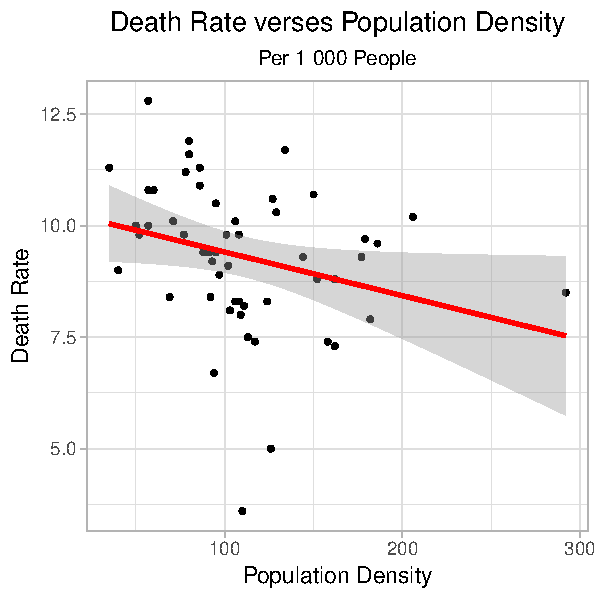
\includegraphics{report_files/figure-latex/fitted_val_plot-1} \end{center}

As can be seen by the above plot, the model was not able to accurately
model individual observations due to the high variance within the data.
This is supported by the model's low Adjusted \(R^2\) value of
\(0.05897\). However, the model was able to capture the decreasing trend
in the data and can be used to draw inference on it.

\section{Plots of Distributions of Parameter Estimates using
Bootstrapping}\label{plots-of-distributions-of-parameter-estimates-using-bootstrapping}

Now it will be examined how sensitive our parameters estimates are with
respect to changes in the data by using bootstrapping.

\begin{center}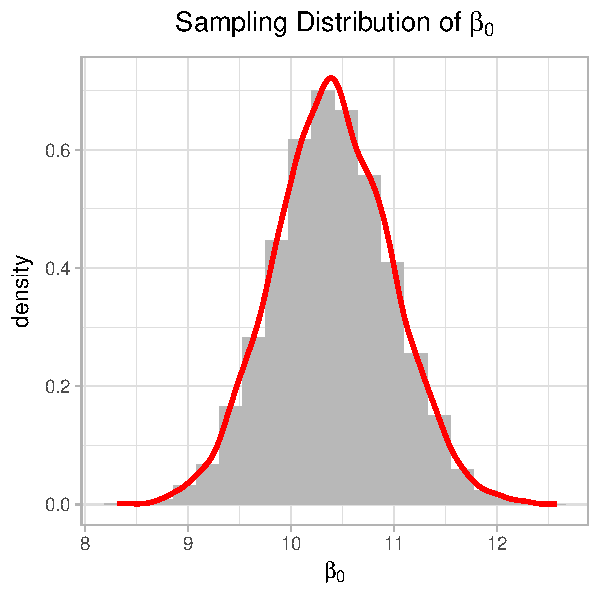
\includegraphics{report_files/figure-latex/plot_beta_0-1} \end{center}

As can be seen by the above plot (and as per theory), the intercept
coefficient appears to be asymptotically Normally distributed with a
mean around \(10.4\). It appears to be quite robust against changes in
the data with an approximate lower and upper bound of \(8.5\) and
\(12.2\) respectively.

\begin{center}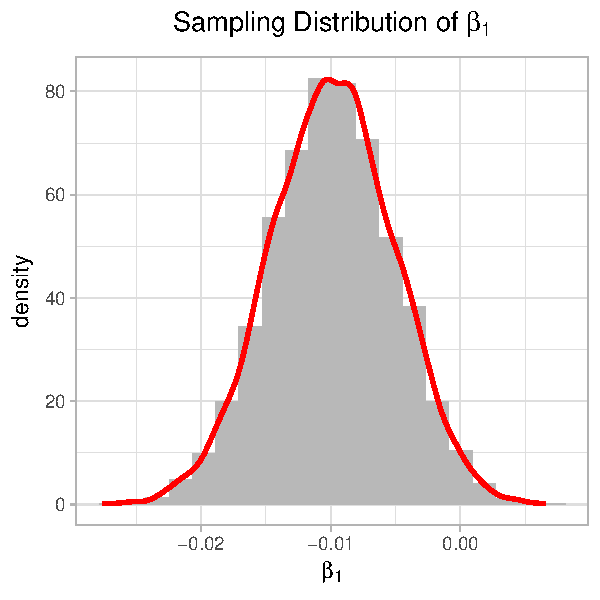
\includegraphics{report_files/figure-latex/plot_beta_1-1} \end{center}

The coefficient of the Population Density covariate also appears to be
asymptotically Normally distributed with a mean around \(-0.01\). This
estimate also appears to be robust against changes in the data with
lower and upper bounds of \(-0.025\) and \(0.005\) respectively.

Thus, based on the above results, the parameter estimates appear to be
quite robust against changes in the data.

\section{Conclusion}\label{conclusion}

In conclusion, there is a decreasing trend between the Death Rate and
Population Density which is attributable to larger towns having access
to more medical services and more medical practitioners than smaller
towns in America. Furthermore, the model was able to accurately pick up
this trend. However, it was not able to accurately predict individual
outcomes.

\section{Appendix}\label{appendix}

\subsection{Code}\label{code}

\subsubsection{Importing the data}\label{importing-the-data}

\begin{Shaded}
\begin{Highlighting}[]
\NormalTok{health.dat <-}\StringTok{ }\KeywordTok{read.delim2}\NormalTok{(}\StringTok{"~/Statistics/Practise_Health_Data/Health_Data.txt"}\NormalTok{)}
\KeywordTok{colnames}\NormalTok{(health.dat) <-}\StringTok{ }\KeywordTok{c}\NormalTok{(}\StringTok{"Death.Rate"}\NormalTok{, }\StringTok{"Doctor.Availability"}\NormalTok{, }\StringTok{"Hospital.Availability"}\NormalTok{, }
    \StringTok{"Annual.Income"}\NormalTok{, }\StringTok{"Population.Density"}\NormalTok{)}
\end{Highlighting}
\end{Shaded}

\subsubsection{Drawing the Scatter Plot
Matrix}\label{drawing-the-scatter-plot-matrix}

\begin{Shaded}
\begin{Highlighting}[]
\KeywordTok{library}\NormalTok{(car)}
\KeywordTok{spm}\NormalTok{(health.dat)}
\end{Highlighting}
\end{Shaded}

\subsubsection{Performing All Subsets Regression and Plotting the
Output}\label{performing-all-subsets-regression-and-plotting-the-output}

\begin{Shaded}
\begin{Highlighting}[]
\KeywordTok{library}\NormalTok{(leaps)}
\NormalTok{leaps.output <-}\StringTok{ }\KeywordTok{regsubsets}\NormalTok{(Death.Rate }\OperatorTok{~}\StringTok{ }\NormalTok{Doctor.Availability }\OperatorTok{+}\StringTok{ }\NormalTok{Hospital.Availability }\OperatorTok{+}\StringTok{ }
\StringTok{    }\NormalTok{Annual.Income }\OperatorTok{+}\StringTok{ }\NormalTok{Population.Density, }\DataTypeTok{data =}\NormalTok{ health.dat, }\DataTypeTok{nbest =} \DecValTok{1}\NormalTok{, }\DataTypeTok{nvmax =} \OtherTok{NULL}\NormalTok{, }
    \DataTypeTok{force.in =} \OtherTok{NULL}\NormalTok{, }\DataTypeTok{force.out =} \OtherTok{NULL}\NormalTok{, }\DataTypeTok{intercept =} \OtherTok{TRUE}\NormalTok{, }\DataTypeTok{method =} \StringTok{"exhaustive"}\NormalTok{)}
\CommentTok{# Plot output (darker colors = lower bic)}
\KeywordTok{plot}\NormalTok{(leaps.output, }\DataTypeTok{scale =} \StringTok{"bic"}\NormalTok{, }\DataTypeTok{main =} \StringTok{"Heatmap of BIC Values"}\NormalTok{, }\DataTypeTok{col =} \KeywordTok{c}\NormalTok{(}\StringTok{"royalblue4"}\NormalTok{, }
    \StringTok{"royalblue3"}\NormalTok{, }\StringTok{"royalblue2"}\NormalTok{, }\StringTok{"royalblue1"}\NormalTok{), }\DataTypeTok{ylab =} \StringTok{"BIC"}\NormalTok{)}
\end{Highlighting}
\end{Shaded}

\subsubsection{Fitting the Linear
Model}\label{fitting-the-linear-model-1}

\begin{Shaded}
\begin{Highlighting}[]
\NormalTok{mod1 <-}\StringTok{ }\KeywordTok{lm}\NormalTok{(Death.Rate }\OperatorTok{~}\StringTok{ }\NormalTok{Population.Density, }\DataTypeTok{data =}\NormalTok{ health.dat)}
\NormalTok{output <-}\StringTok{ }\KeywordTok{coef}\NormalTok{(}\KeywordTok{summary}\NormalTok{(mod1))}
\NormalTok{knitr}\OperatorTok{::}\KeywordTok{kable}\NormalTok{(output, }\DataTypeTok{caption =} \StringTok{"Fitted Values and their Statistics for the Fitted Model"}\NormalTok{)}
\end{Highlighting}
\end{Shaded}

\subsubsection{Plotting the Residuals}\label{plotting-the-residuals}

\begin{Shaded}
\begin{Highlighting}[]
\KeywordTok{autoplot}\NormalTok{(mod1, }\DataTypeTok{smooth.colour =} \StringTok{"red"}\NormalTok{, }\DataTypeTok{ad.colour =} \StringTok{"blue"}\NormalTok{, }\DataTypeTok{size =} \FloatTok{0.9}\NormalTok{) }\OperatorTok{+}\StringTok{ }\KeywordTok{theme_light}\NormalTok{() }\OperatorTok{+}\StringTok{ }
\StringTok{    }\KeywordTok{theme}\NormalTok{(}\DataTypeTok{plot.title =} \KeywordTok{element_text}\NormalTok{(}\DataTypeTok{hjust =} \FloatTok{0.5}\NormalTok{))}
\end{Highlighting}
\end{Shaded}

\subsubsection{Plotting the Fitted
Values}\label{plotting-the-fitted-values}

\begin{Shaded}
\begin{Highlighting}[]
\KeywordTok{ggplot}\NormalTok{(}\DataTypeTok{data =} \KeywordTok{data.frame}\NormalTok{(}\DataTypeTok{x =}\NormalTok{ health.dat}\OperatorTok{$}\NormalTok{Population.Density, }\DataTypeTok{y =}\NormalTok{ health.dat}\OperatorTok{$}\NormalTok{Death.Rate), }
    \DataTypeTok{mapping =} \KeywordTok{aes}\NormalTok{(x, y)) }\OperatorTok{+}\StringTok{ }\KeywordTok{geom_point}\NormalTok{(}\DataTypeTok{size =} \FloatTok{0.9}\NormalTok{) }\OperatorTok{+}\StringTok{ }\KeywordTok{geom_smooth}\NormalTok{(}\DataTypeTok{data =} \KeywordTok{data.frame}\NormalTok{(}\DataTypeTok{x =}\NormalTok{ health.dat}\OperatorTok{$}\NormalTok{Population.Density, }
    \DataTypeTok{y =}\NormalTok{ health.dat}\OperatorTok{$}\NormalTok{Death.Rate), }\DataTypeTok{mapping =} \KeywordTok{aes}\NormalTok{(x, y), }\DataTypeTok{method =} \StringTok{"lm"}\NormalTok{, }\DataTypeTok{formula =}\NormalTok{ y }\OperatorTok{~}\StringTok{ }
\StringTok{    }\NormalTok{x }\OperatorTok{+}\StringTok{ }\DecValTok{1}\NormalTok{, }\DataTypeTok{col =} \StringTok{"red"}\NormalTok{, }\DataTypeTok{size =} \DecValTok{1}\NormalTok{) }\OperatorTok{+}\StringTok{ }\KeywordTok{ggtitle}\NormalTok{(}\StringTok{"Death Rate verses Population Density"}\NormalTok{, }
    \DataTypeTok{subtitle =} \StringTok{"Per 1 000 People"}\NormalTok{) }\OperatorTok{+}\StringTok{ }\KeywordTok{xlab}\NormalTok{(}\StringTok{"Population Density"}\NormalTok{) }\OperatorTok{+}\StringTok{ }\KeywordTok{ylab}\NormalTok{(}\StringTok{"Death Rate"}\NormalTok{) }\OperatorTok{+}\StringTok{ }
\StringTok{    }\KeywordTok{theme_light}\NormalTok{() }\OperatorTok{+}\StringTok{ }\KeywordTok{theme}\NormalTok{(}\DataTypeTok{plot.title =} \KeywordTok{element_text}\NormalTok{(}\DataTypeTok{hjust =} \FloatTok{0.5}\NormalTok{), }\DataTypeTok{plot.subtitle =} \KeywordTok{element_text}\NormalTok{(}\DataTypeTok{hjust =} \FloatTok{0.5}\NormalTok{))}
\end{Highlighting}
\end{Shaded}

\subsubsection{Performing Bootstrapping and Plotting the
Results}\label{performing-bootstrapping-and-plotting-the-results}

\begin{Shaded}
\begin{Highlighting}[]
\NormalTok{b_}\DecValTok{0}\NormalTok{ <-}\StringTok{ }\NormalTok{mod1}\OperatorTok{$}\NormalTok{coefficients[}\DecValTok{1}\NormalTok{]}
\NormalTok{b_}\DecValTok{1}\NormalTok{ <-}\StringTok{ }\NormalTok{mod1}\OperatorTok{$}\NormalTok{coefficients[}\DecValTok{2}\NormalTok{]}
\NormalTok{smod1 <-}\StringTok{ }\KeywordTok{summary}\NormalTok{(mod1)}
\NormalTok{sig <-}\StringTok{ }\NormalTok{smod1}\OperatorTok{$}\NormalTok{sigma}
\NormalTok{bootstrap_param_estimates <-}\StringTok{ }\ControlFlowTok{function}\NormalTok{() \{}
\NormalTok{    e_r <-}\StringTok{ }\KeywordTok{rnorm}\NormalTok{(}\KeywordTok{length}\NormalTok{(health.dat}\OperatorTok{$}\NormalTok{Population.Density), }\DataTypeTok{mean =} \DecValTok{0}\NormalTok{, }\DataTypeTok{sd =}\NormalTok{ sig)}
\NormalTok{    y_r <-}\StringTok{ }\NormalTok{b_}\DecValTok{0} \OperatorTok{+}\StringTok{ }\NormalTok{b_}\DecValTok{1} \OperatorTok{*}\StringTok{ }\NormalTok{health.dat}\OperatorTok{$}\NormalTok{Population.Density }\OperatorTok{+}\StringTok{ }\NormalTok{e_r}
\NormalTok{    mod_r <-}\StringTok{ }\KeywordTok{lm}\NormalTok{(y_r }\OperatorTok{~}\StringTok{ }\NormalTok{health.dat}\OperatorTok{$}\NormalTok{Population.Density)}
    \KeywordTok{return}\NormalTok{(mod_r}\OperatorTok{$}\NormalTok{coefficients)}
\NormalTok{\}}

\NormalTok{params_samp <-}\StringTok{ }\KeywordTok{matrix}\NormalTok{(}\KeywordTok{replicate}\NormalTok{(}\DecValTok{7500}\NormalTok{, }\KeywordTok{bootstrap_param_estimates}\NormalTok{()), }\DataTypeTok{ncol =} \DecValTok{2}\NormalTok{, }
    \DataTypeTok{byrow =} \OtherTok{TRUE}\NormalTok{)}

\NormalTok{b_0_vals <-}\StringTok{ }\NormalTok{params_samp[, }\DecValTok{1}\NormalTok{]}
\NormalTok{b_1_vals <-}\StringTok{ }\NormalTok{params_samp[, }\DecValTok{2}\NormalTok{]}

\KeywordTok{ggplot}\NormalTok{(}\DataTypeTok{data =} \KeywordTok{data.frame}\NormalTok{(}\DataTypeTok{x =}\NormalTok{ b_0_vals), }\DataTypeTok{mapping =} \KeywordTok{aes}\NormalTok{(x)) }\OperatorTok{+}\StringTok{ }\KeywordTok{geom_histogram}\NormalTok{(}\DataTypeTok{bins =} \DecValTok{20}\NormalTok{, }
    \DataTypeTok{fill =} \StringTok{"gray72"}\NormalTok{, }\KeywordTok{aes}\NormalTok{(}\DataTypeTok{y =}\NormalTok{ ..density..)) }\OperatorTok{+}\StringTok{ }\KeywordTok{stat_density}\NormalTok{(}\DataTypeTok{geom =} \StringTok{"line"}\NormalTok{, }\DataTypeTok{col =} \StringTok{"red"}\NormalTok{, }
    \DataTypeTok{size =} \DecValTok{1}\NormalTok{) }\OperatorTok{+}\StringTok{ }\KeywordTok{ggtitle}\NormalTok{(}\DataTypeTok{label =} \KeywordTok{expression}\NormalTok{(}\KeywordTok{paste}\NormalTok{(}\StringTok{"Sampling Distribution of "}\NormalTok{, }
\NormalTok{    beta[}\DecValTok{0}\NormalTok{]))) }\OperatorTok{+}\StringTok{ }\KeywordTok{xlab}\NormalTok{(}\KeywordTok{expression}\NormalTok{(}\KeywordTok{paste}\NormalTok{(beta[}\DecValTok{0}\NormalTok{]))) }\OperatorTok{+}\StringTok{ }\KeywordTok{theme_light}\NormalTok{() }\OperatorTok{+}\StringTok{ }\KeywordTok{theme}\NormalTok{(}\DataTypeTok{plot.title =} \KeywordTok{element_text}\NormalTok{(}\DataTypeTok{hjust =} \FloatTok{0.5}\NormalTok{))}

\KeywordTok{ggplot}\NormalTok{(}\DataTypeTok{data =} \KeywordTok{data.frame}\NormalTok{(}\DataTypeTok{x =}\NormalTok{ b_1_vals), }\DataTypeTok{mapping =} \KeywordTok{aes}\NormalTok{(x)) }\OperatorTok{+}\StringTok{ }\KeywordTok{geom_histogram}\NormalTok{(}\DataTypeTok{bins =} \DecValTok{20}\NormalTok{, }
    \DataTypeTok{fill =} \StringTok{"gray72"}\NormalTok{, }\KeywordTok{aes}\NormalTok{(}\DataTypeTok{y =}\NormalTok{ ..density..)) }\OperatorTok{+}\StringTok{ }\KeywordTok{stat_density}\NormalTok{(}\DataTypeTok{geom =} \StringTok{"line"}\NormalTok{, }\DataTypeTok{col =} \StringTok{"red"}\NormalTok{, }
    \DataTypeTok{size =} \DecValTok{1}\NormalTok{) }\OperatorTok{+}\StringTok{ }\KeywordTok{ggtitle}\NormalTok{(}\KeywordTok{expression}\NormalTok{(}\KeywordTok{paste}\NormalTok{(}\StringTok{"Sampling Distribution of "}\NormalTok{, beta[}\DecValTok{1}\NormalTok{]))) }\OperatorTok{+}\StringTok{ }
\StringTok{    }\KeywordTok{xlab}\NormalTok{(}\KeywordTok{expression}\NormalTok{(}\KeywordTok{paste}\NormalTok{(beta[}\DecValTok{1}\NormalTok{]))) }\OperatorTok{+}\StringTok{ }\KeywordTok{theme_light}\NormalTok{() }\OperatorTok{+}\StringTok{ }\KeywordTok{theme}\NormalTok{(}\DataTypeTok{plot.title =} \KeywordTok{element_text}\NormalTok{(}\DataTypeTok{hjust =} \FloatTok{0.5}\NormalTok{))}
\end{Highlighting}
\end{Shaded}

\section*{Bibliography}\label{bibliography}
\addcontentsline{toc}{section}{Bibliography}

\hypertarget{refs}{}
\hypertarget{ref-houghtonMifflin2018}{}
Houghton Mifflin Harcourt. 2018. \emph{Data for Linear Regression:
Health}. ed. Houghton Mifflin Harcourt. Available:
\url{https://college.cengage.com/mathematics/brase/understandable_statistics/7e/students/datasets/mlr/frames/mlr07.html}
{[}2018, February 15{]}.


\end{document}
